\scanpage{69}
% archive foliation: 68
l'anneau de $\underline W^a(\mathfrak X)$ est engendré par $\unsure{v}r$ générateurs sur celui de $S$.

Dans le cas général \inserted{($S$ affine)}, on a $C=\varinjlim C_i$, où les $C_i$ sont des ss-$W(A)$-algèbres \inserted{de type fini} de $C$. On a donc, pour $T$ affine
% The written argument order and the curved transposition stroke are both retained.
\[
\begin{aligned}
\mathrm{Hom}_{\underline W(S)}\text{\figure{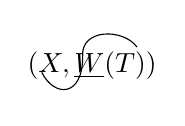
\begin{tikzpicture}[baseline=(args.base)]
\node[inner sep=0pt] (args) {$(\mathfrak X,\underline W(T))$};
\draw (-.64,-.08) .. controls (-.48,-.40) and (-.12,-.40) .. (-.12,.12) .. controls (-.15,.48) and (.40,.48) .. (.57,.24);
\end{tikzpicture}}}
&=\mathrm{Hom}_{W(A)\text{-alg}}(\deleted{\unsure{W(B)}}C,\underline W(B))\\
&\simeq\varprojlim\mathrm{Hom}_{\underline W(A)\text{-alg}}(C_i,\underline W(B))\\
&\simeq\varprojlim\mathrm{Hom}_{A\text{-alg}}(\underline W^a(C_i),B)\\
&\simeq\mathrm{Hom}_{A\text{-alg}}(\varinjlim\underline W^a(C_i),B)
\end{aligned}
\]
Soit donc
\[
\varinjlim W^a(C_i)=\deleted{\unsure{W^a}}D\qquad\deleted{\unsure{\longrightarrow}}
\]
on a obtenu un isom fonctoriel
\[
\mathrm{Hom}_{\underline W(S)}(\underline W(T),\mathfrak X)\simeq\mathrm{Hom}_S(T,\operatorname{Spec}(D)),
\]
d'où le résultat.

\inserted{\uline{Corollaire} Dans les conditions précédentes, si $\mathfrak X\xrightarrow{f}\mathfrak Y$ est un morphisme \deleted{affine} de $S$-préschémas affines qui est de type fini (resp. une immersion fermée)}
\margin{alors $\underline W^a(f)$ est un morphisme \uline{affine} de type fini pourvu que $W/S$ \unsure{soit} de type fini. resp. une immersion fermée}

\deleted{\uline{Corollaire} Soit $f:\mathfrak X\to\mathfrak Y$ un morphisme de $\underline W(S)$-préschémas, $\unsure{S}$ supposons que $\underline W^a(\mathfrak X)$ et $\underline W^a(\mathfrak Y)$ existent, alors $W$ $W^a(f):W^a(\mathfrak X)\unsure{-|\to}W^a(\mathfrak Y)$ est affine,}
